\newpage
\section{Лабораторная работа 3 (вариант 5-8)}

\subsection{Задание}
Цель работы - создание программы, реализующей искусственный нейрон; разработка процедуры обучения нейрона; использование полученных результатов для решения тестовых задач классификации и аппроксимации.

\subsection{WTA нейрон}
Нейроны типа WTA (Winner Takes All — победитель получает все) всегда используются группами, в которых конкурируют между собой. Структурная схема группы (слоя) нейронов типа WTA представлена на рисунке ниже (рисунок \ref{img:wta}).

\begin{figure}[H]
\centering
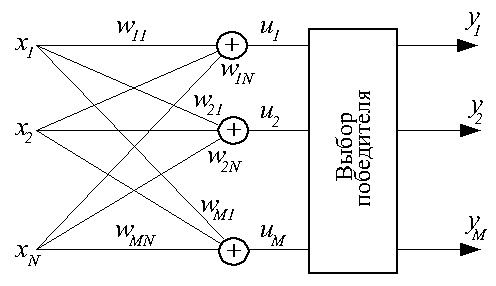
\includegraphics[scale=0.5]{wta.png}
\caption{Структурная схема слоя нейрона типа WTA}
\label{img:wta}
\end{figure}

Каждый конкурирующий нейрон в группе получает одни и те же входные сигналы. Каждый нейрон рассчитывает выходной сигнал своего сумматора обычным образом:

\begin{equation}\label{eq:Func}
	u_i=\sum\limits_{j=0}^N w_{ij} x_j.
\end{equation}

\begin{itemize}
\item По результатам сравнения всех $u_i, j=1, 2, ..., M$ выбирается нейрон-победитель, обладающий наибольшим значением $u_i$. Выходной сигнал $y_i$ нейрона-победителя получает значение 1, выходные сигналы всех остальных нейронов — 0.
\end{itemize}

Для обучения нейронов типа WTA не требуется учитель, оно практически полностью аналогично обучению инстара Гроссберга. Начальные значения весовых коэффициентов всех нейронов выбираются случайным образом с последующей нормализацией относительно 1.
При предъявлении каждого обучающего вектора $X^k$ определяется нейрон-победитель, что дает ему право уточнить свои весовые коэффициенты по упрощенному (в силу бинарности $y_i$) правилу Гроссберга:

\begin{equation}\label{eq:Func}
    w_{ij}(t+1)=w_{ij}(t)+\eta(x_j^k-w_{ij}(t)).
\end{equation}
Все проигравшие нейроны оставляют свои весовые коэффициенты неизменными. 

В каждом цикле обучения побеждает тот нейрон, чей текущий вектор входных весов $W_i$ наиболее близок входному вектору $X_k$. При этом вектор $W_i$ корректируется в сторону вектора $X_k$. Поэтому в ходе обучения каждая группа близких друг другу входных векторов (кластер) обслуживается отдельным нейроном.




Понятие «близости» двух векторов можно продемонстрировать на следующем примере. Пусть на очередной итерации обучения сети в режиме «онлайн» имеется входной вектор $X^k$. Тогда вычисление взвешенной суммы для i-го нейрона осуществляется по формуле:
\begin{equation}\label{eq:sum_func}
    u _ { i } = W _ { i } ^ { T } \cdot X ^ { k } = \sum _ { j = 1 } ^ { N } w _ { i j } \cdot x _ { j } ^ { k } = \left\| W _ { i } ^ { T } \right\| \cdot \left\| X ^ { k } \right\| \cdot \cos \left( \sphericalangle   W _ { i } , X ^ { k } \right)
\end{equation}

Поскольку вектора $W_i$ и $X^k$ нормализованы, то взвешенная сумма i-го нейрона равна косинусу угла между вектором весов и входным вектором. На рис. \ref{img:angle} представлена геометрическая интерпретация. Чем ближе весовой вектор ко входному, тем ближе косинус угла между векторами к 1.

\begin{figure}[H]
\centering
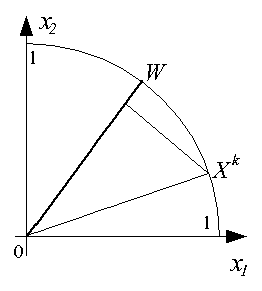
\includegraphics[scale=0.5]{angle.png}
\caption{Геометрическая интерпретация весов нейронов}
\label{img:angle}
\end{figure}

В режиме кластеризации при подаче на вход слоя нейронов типа WTA очередного вектора $X^k$ определяется степень его близости к векторам $W_i$ в виде косинусов углов между этими векторами, после чего определяется наиболее «близкий» вектор весов, отвечающий за тот или иной кластер.

Результат обучения слоя нейронов типа WTA на последовательности девяти двухкомпонентных входных векторов ${X^1, X^2, ..., X^9}$ иллюстрирует (рис. \ref{img:wta_teached}). Здесь были выделены три кластера входных векторов $\{X^1, X^8\}$, $\{X^3, X^4, X^5\}$ и $\{X^2, X^6, X^7, X^9\}$. За их распознавание отвечают три нейрона с векторами входных весов $W_1$, $W_2$ и $W_3$ соответственно.

\begin{figure}[H]
\centering
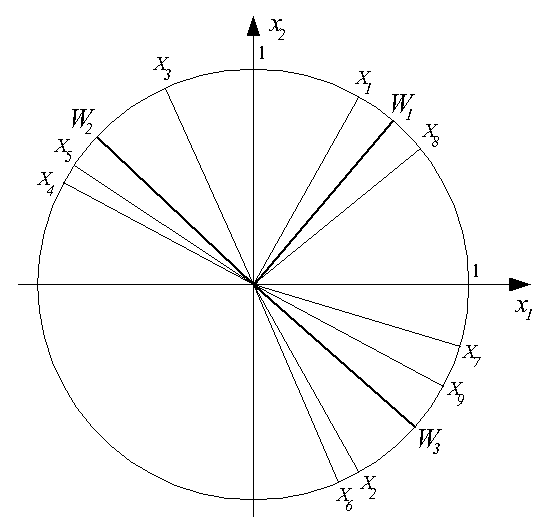
\includegraphics[scale=0.4]{wta_teached.png}
\caption{Результат обучения слоя нейронов типа WTA}
\label{img:wta_teached}
\end{figure}

Серьезная проблема в использовании нейронов типа WTA — возможность возникновения "мертвых" нейронов, т.е. нейронов, ни разу не победивших в конкурентной борьбе в ходе обучения и поэтому оставшихся в начальном состоянии. Для исключения "ложных" срабатываний в режиме классификации мертвые нейроны после окончания обучения должны быть удалены.

Для уменьшения количества мертвых нейронов (и, следовательно, повышения точности распознавания) используется модифицированное обучение, основанное на учете числа побед нейронов и шрафовании наиболее "зарвавшихся" среди них. Дисквалификация может быть реализована либо назначением порога числа побед, после которого слишком активный нейрон "засыпает" на заданное число циклов обучения, либо искусственным уменьшением величины  пропорционально числу побед.



\subsection{Исходные данные}

Обучающие данные для варианта 8 представлены на рисунке \ref{img:train_sphere}.

\begin{figure}[H]
\centering
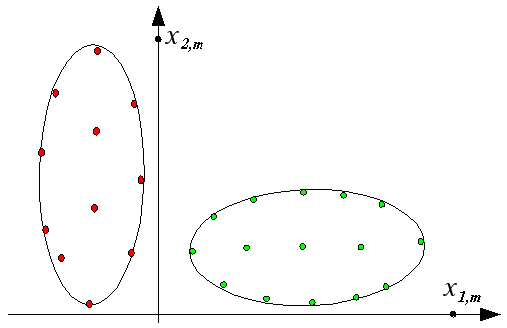
\includegraphics[scale=0.6]{train_sphere.png}
\caption{Данные для обучения варианта 8}
\label{img:train_sphere}
\end{figure}

\subsection{Обучение}

Для обучения были сгенерированы в случайном порядке точки, принадлежашие двум областям (рис. \ref{img:points}, а). После этого вектор входных значений, состоящих из координат точек, был нормализован (рис. \ref{img:points}, б) по формуле:
\begin{equation}\label{eq:normaFunc}
	x_{j}\leftarrow\frac{x_{j}}{\sqrt{x_{1}^{2}+x_{2}^{2}+\ldots+x_{N}^{2}}}.
\end{equation}

%\begin{figure}[h]
%    \begin{center}
%        \begin{minipage}[h]{0.48\linewidth}
%            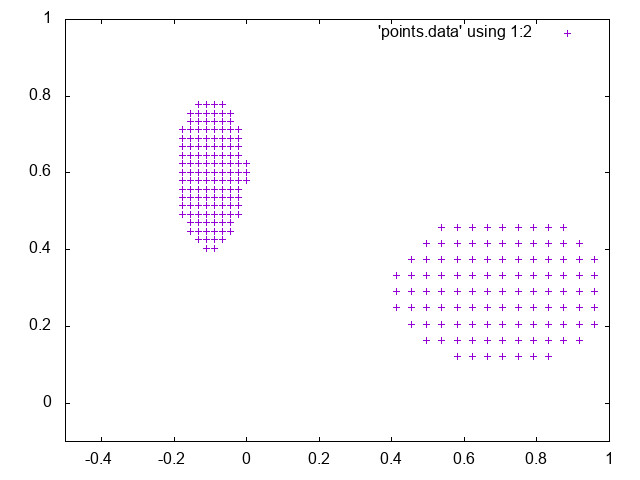
\includegraphics[width=1\linewidth]{points_nonorma.jpg}
%            %\caption{Обучающие данные} %% подпись к рисунку
%            \label{img:points} %% метка рисунка для ссылки на него
%        \end{minipage}
%        \hfill 
%        \begin{minipage}[h]{0.48\linewidth}
%            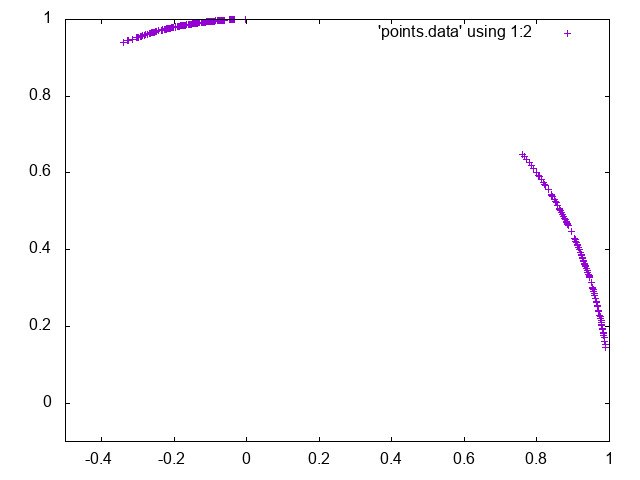
\includegraphics[width=1\linewidth]{points.png}
%            %\caption{Обчающие данные нормализованные}
%            \label{img:points_norma}
%        \end{minipage}
%        \begin{minipage}[h]{1\linewidth}
%            \centering
%            \begin{tabular}{p{0.50\linewidth}p{0.40\linewidth}}
%                %\centering % Обчающие данные после нормализации &
%                    \caption{Обучающие данные} &
%                %\centering %Обчающие данные после нормализации \\
%                    \caption{Обчающие данные после нормализации} \\
%            \end{tabular}
%        \end{minipage}
%    \end{center}
%\end{figure}


\begin{figure}[h]
    \begin{minipage}[h]{0.49\linewidth}
        \center{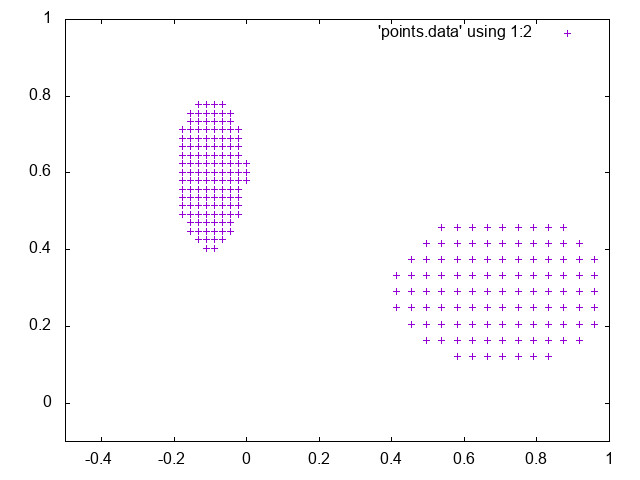
\includegraphics[width=1\linewidth]{points_nonorma.jpg} \\ а)}
    \end{minipage}
    \hfill
    \begin{minipage}[h]{0.49\linewidth}
        \center{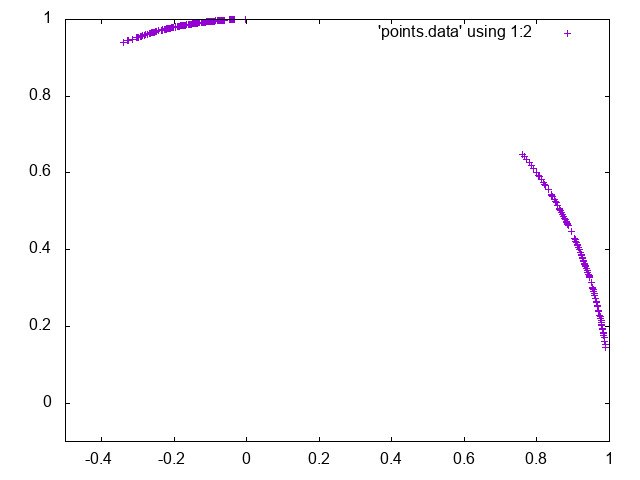
\includegraphics[width=1\linewidth]{points.png} \\ б)}
    \end{minipage}
    \caption{Обучающие данные}
    \label{img:points}
\end{figure}


Оба множнста имеют примерно одинаковое количесво точек. Это сделано, чтобы не допусть паревеса весов в сторону какого-либо из множеств.

Параметры обучения:
\begin{itemize}
    \item Размерность входных векторов: 2
    \item Количество нейронов: 4
    \item Количество эпох обучения: 2
    \item Коэффициент обучения $\eta$: 0,1
    \item Коэффициент штрафа при обучении: 0,01
    \item Начальные значения весов: (-1, -1) для всех весов
\end{itemize}

Обучение проводилось онлайн-методом - корректировка весов проводилась после подачи каджого входного вектора.

Коэффициент штрафа при обучении необходим для решения проблемы «мертвых» нейронов. Для каждого нейрона в слое вводится счетчик побед. Он изменяется на каждой итерации обучения для нейронов-победителей. Считчик используется для коррекции взвешенных сумм нейронов перед процедурой определения нейрона-победителя. Взвешенная сумма каждого нейрона рассчитывается по формуле:
\begin{equation}\label{eq:penaltyFunc}
    u _ { i } = \left( \sum _ { j = 1 } ^ { N } w _ { i j } \cdot x _ { j } \right) - p \cdot C_i,
\end{equation}
где $C_i, i=1, 2, ..., M$ - счетчик побед, p - коэффициент штрафа при обучении.\\
%\vspace{\baselineskip}
~\\
  У WTA-нейрона нет понятия расстояния до входного вектора в отличие от самоорганизующихся сетей, построенных на WTA-нейронах. Определение победителя происходит исключительно по величине значения взвешенной суммы. То есть, у победителя она оказывается максимальной после предъявления очередного вектора обучения на слой. Только потом уже корректируется вес у этого нейрона-победителя по формеле \ref{eq:Func}. Но, чтобы дать возможность победить другим нейронам, нужно штрафовать победителя слудуюшими способами:

\begin{enumerate} 
  \item Уменьшить взвешенную сумму нейрона-победителя, чтобы при сравнении  взвешенных сумм всех нейронов, она оказалась меньше, чем могла бы быть.
  \item Ввести какой-либо коэффициент, отражающий количество подряд идущих побед нейрона. По предельному значению замораживать его на несколько циклов обучения.
\end{enumerate}
%\vspace{\baselineskip}
В рамках данной лаботароной работы был реализовани первый варинт.

\subsection{Результат}

Результат процесса обучения представлен на рис. \ref{img:result}. Из начального положения $(x_1, x_2) = (-1, -1)$ (рис.\ref{img:result}, a), значения весов векторов постепенно выравниваются и достигаю конечнго распределения, как на рис.\ref{img:result}, б). Сам процесс обучения частично предствлен на рис. \ref{img:teaching}.

\begin{figure}[h]
    \begin{minipage}[h]{0.49\linewidth}
        \center{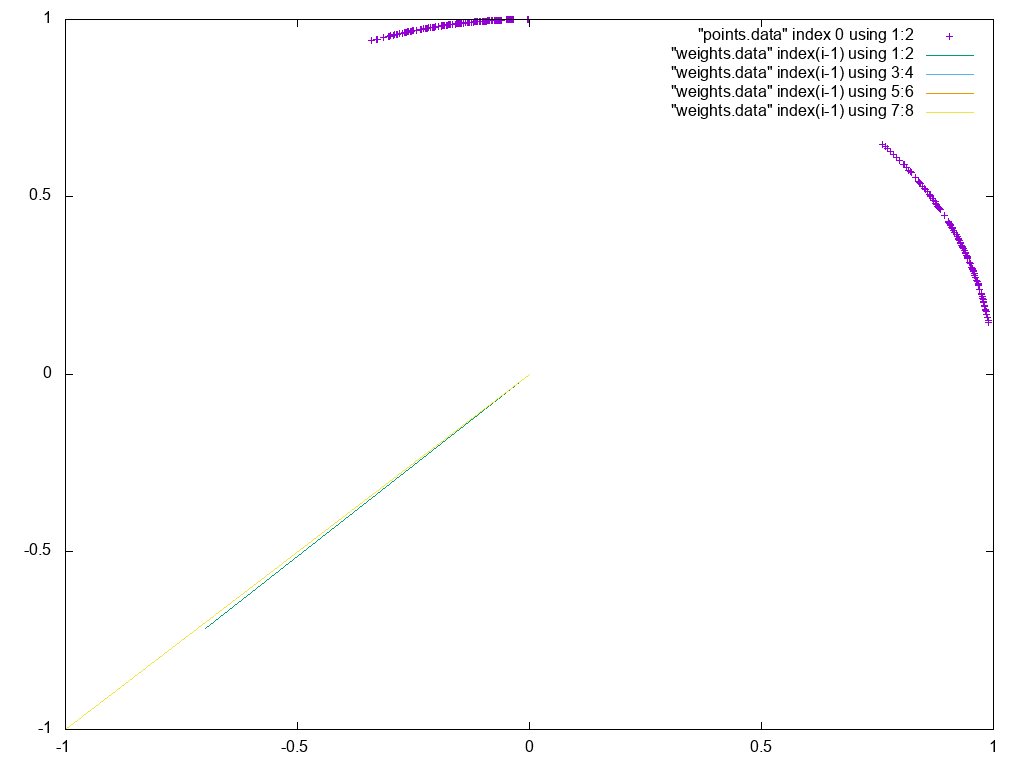
\includegraphics[width=1\linewidth]{train0.png} \\ а)}
    \end{minipage}
    \hfill
    \begin{minipage}[h]{0.49\linewidth}
        \center{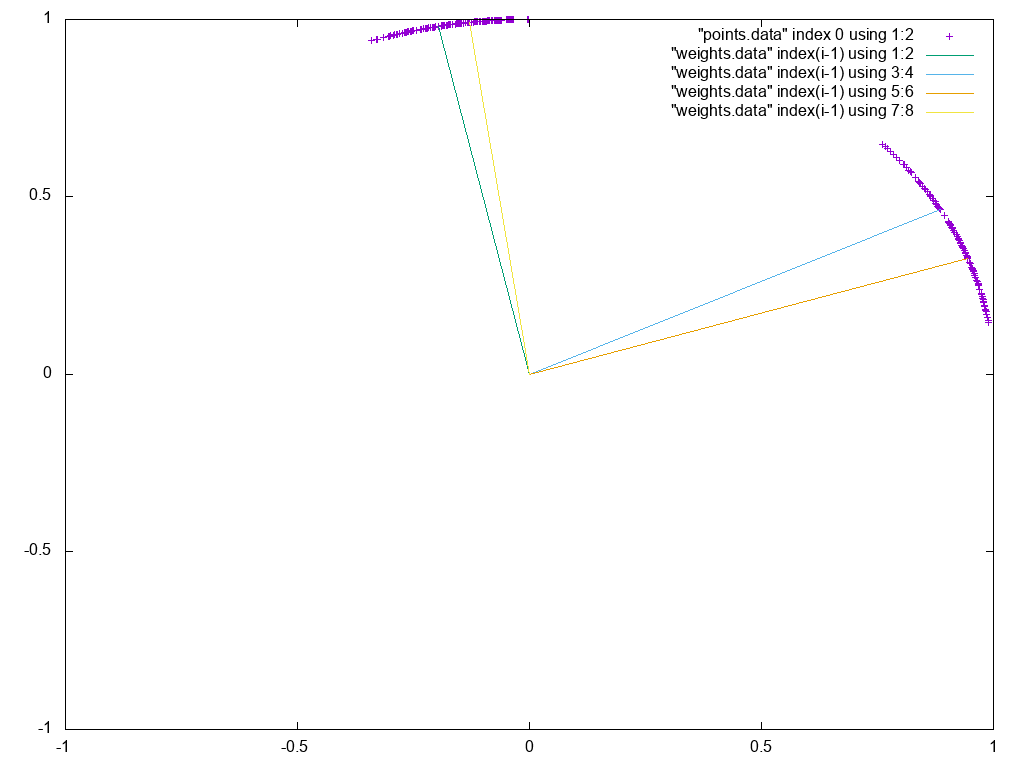
\includegraphics[width=1\linewidth]{train6.png} \\ б)}
    \end{minipage}
    \caption{a) - нулевое положение, б) - конечный результат}
    \label{img:result}
\end{figure}

\begin{figure}[H]
    \begin{minipage}[h]{0.4\linewidth}
        \center{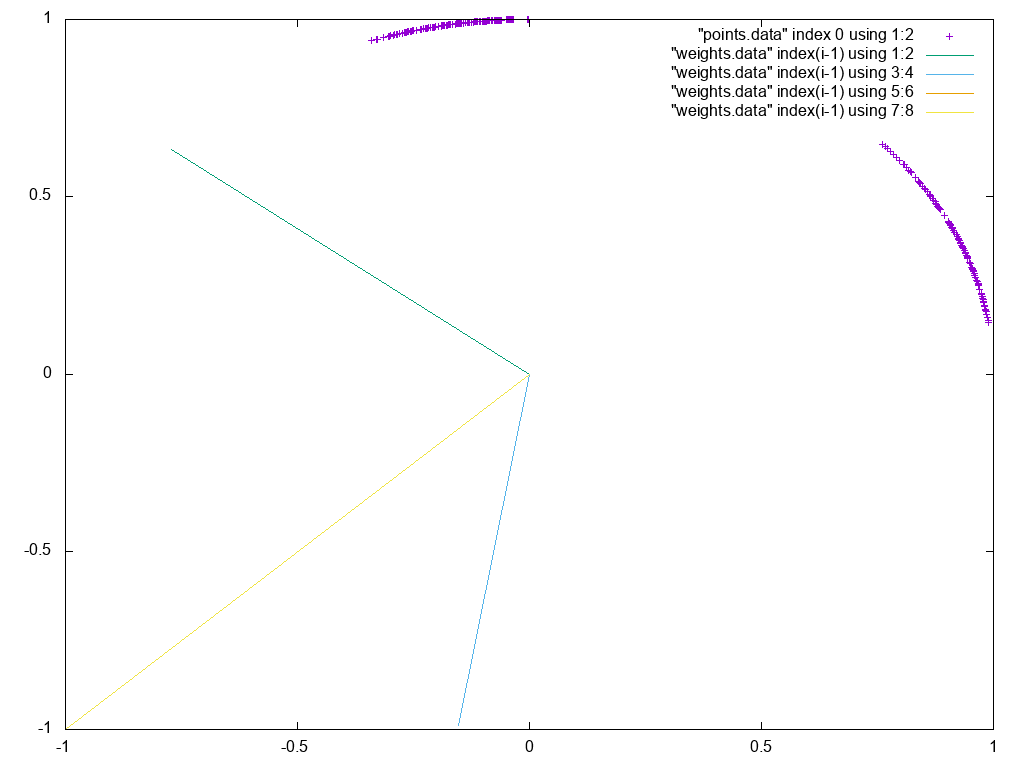
\includegraphics[width=1\linewidth]{train1.png} а)}  \\
    \end{minipage}
    \hfill
    \begin{minipage}[h]{0.4\linewidth}
        \center{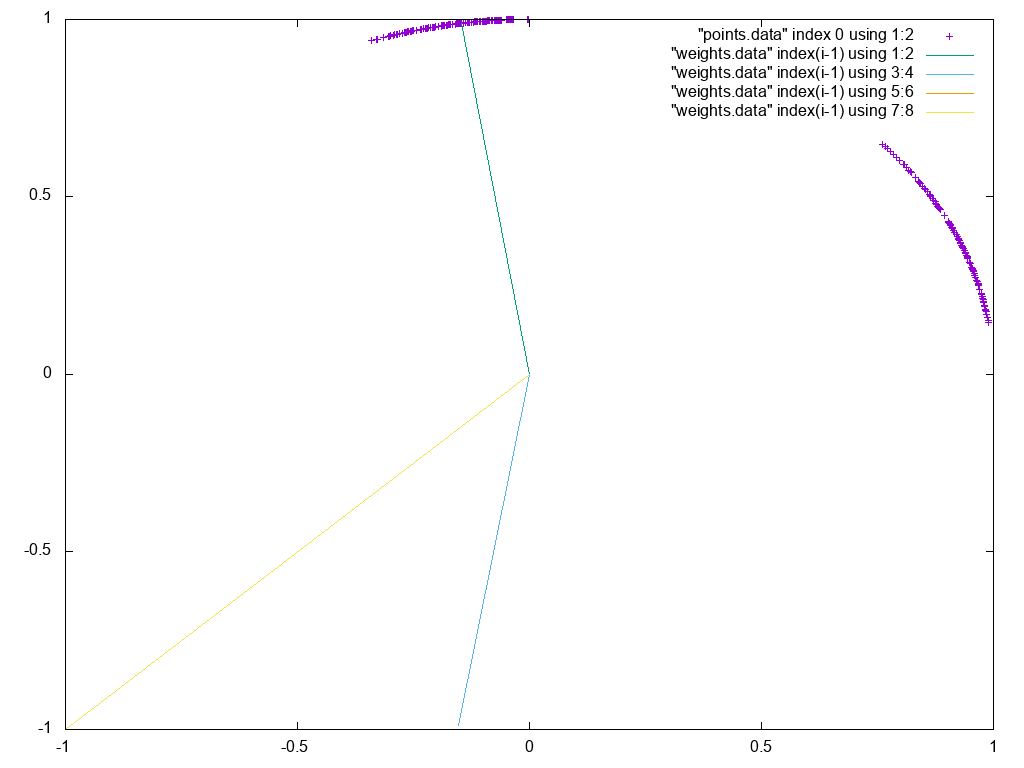
\includegraphics[width=1\linewidth]{train11.png} б)} \\
    \end{minipage}
    \vfill
    \begin{minipage}[h]{0.4\linewidth}
        \center{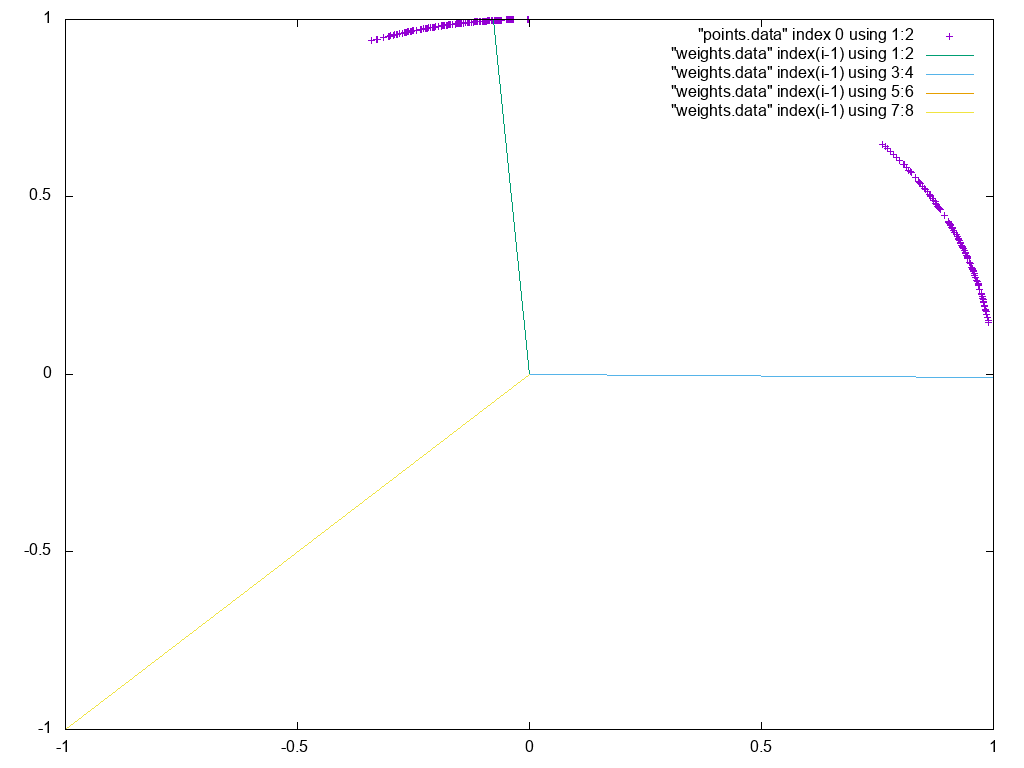
\includegraphics[width=1\linewidth]{train2.png} в)} \\
    \end{minipage}
    \hfill
    \begin{minipage}[h]{0.4\linewidth}
        \center{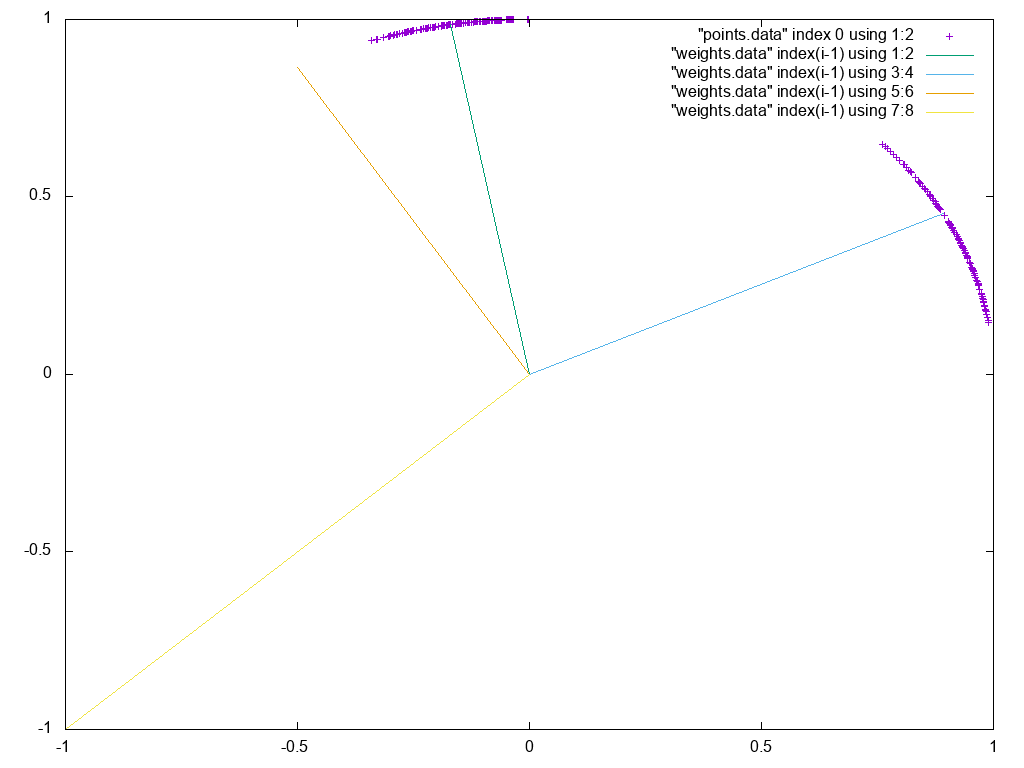
\includegraphics[width=1\linewidth]{train3.png} г)} \\
    \end{minipage}
    \vfill
    \begin{minipage}[h]{0.4\linewidth}
        \center{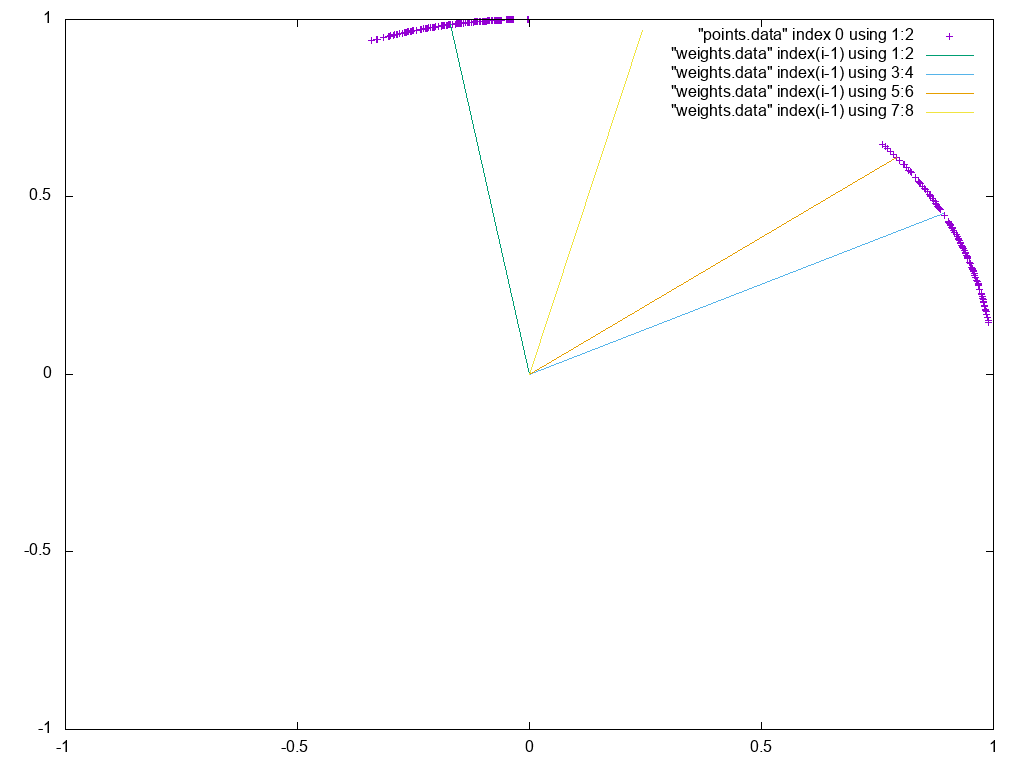
\includegraphics[width=1\linewidth]{train4.png} д)}  \\
    \end{minipage}
    \hfill
    \begin{minipage}[h]{0.4\linewidth}
        \center{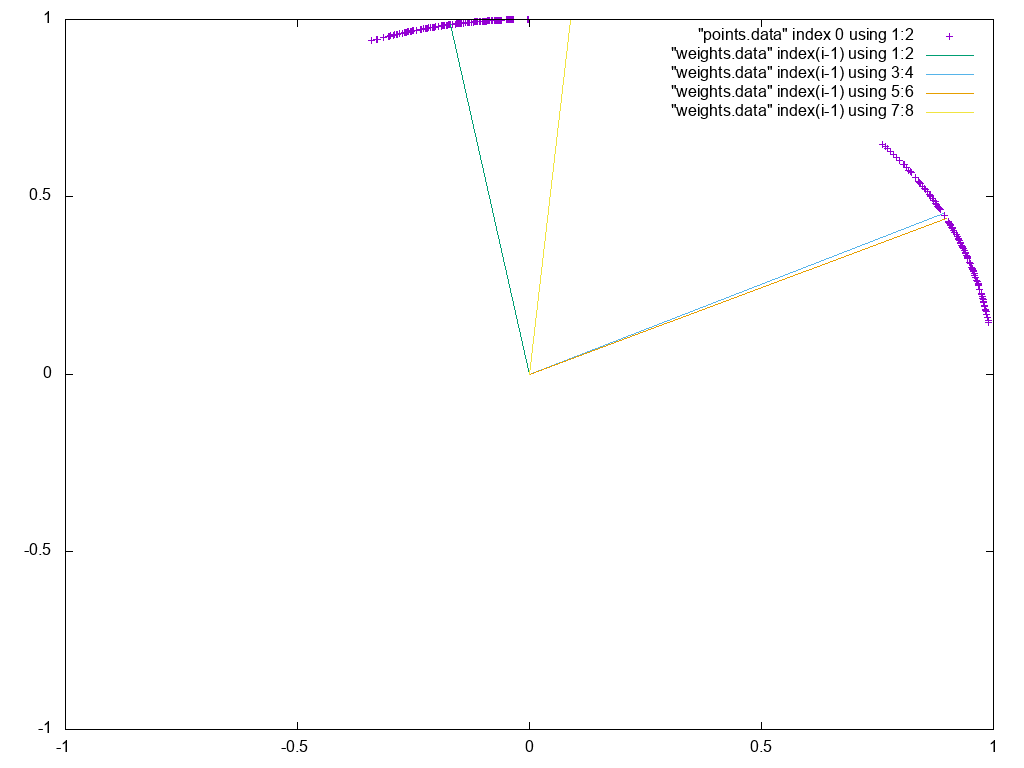
\includegraphics[width=1\linewidth]{train5.png} е)} \\
    \end{minipage}
    \caption{Процесс обучения}
    \label{img:teaching}
\end{figure}


\subsection{Иходный код}
Файл main.cpp
\begin{verbatim}
     1	#include "WTA.h"
     2	#include <algorithm>
     3	#include <cmath>
     4	
     5	void GenerateElipsis2DPointSet(
     6	        std::vector<std::vector<double>> *points,
     7	        double a, double b,
     8	        double xOffset, double yOffset,
     9	        double rotation, double step) {
    10	    a = (a < 0) ? -a : a;
    11	    b = (b < 0) ? -b : b;
    12	    double norm;
    13	
    14	    for (double x = -a; x <= a; x += step) {
    15	        for (double y = -b; y <= b; y += step) {
    16	            if (((x * x) / (a * a) + (y * y) / (b * b)) <= 1) {
    17	                std::vector<double> v(2);
    18	                v[0] = (x * cos(rotation) + y * sin(rotation)) + xOffset
;
    19	                v[1] = (-x * sin(rotation) + y * cos(rotation)) + yOffse
t;
    20	                norm = sqrt(v[0] * v[0] + v[1] * v[1]);
    21	                // normalize
    22	                v[0] /= norm;
    23	                v[1] /= norm;
    24	                points->emplace_back(std::move(v));
    25	            }
    26	        }
    27	    }
    28	
    29	    std::cout << "finish" << std::endl;
    30	}
    31	
    32	std::vector<std::vector<double>> Generate2DTrainSet() {
    33	    std::vector<std::vector<double>> trainSet;
    34	
    35	    GenerateElipsis2DPointSet(&trainSet, 0.3, 0.2, 0.7, 0.3, -M_PI, 0.04
2);
    36	    GenerateElipsis2DPointSet(&trainSet, 0.2, 0.1, -0.1, 0.6, M_PI_2, 0.
022);
    37	
    38	    std::random_shuffle(trainSet.begin(), trainSet.end());
    39	    return trainSet;
    40	}
    41	
    42	void DumpPoints(std::ostream &output, const std::vector<std::vector<doub
le>> &points) {
    43	    for (size_t iPoint = 0; iPoint < points.size(); ++iPoint) {
    44	        for (size_t iCoord = 0; iCoord < points[iPoint].size(); ++iCoord
)
    45	            output << points[iPoint][iCoord] << "\t";
    46	
    47	        output << std::endl;
    48	    }
    49	}
    50	
    51	int main() {
    52	    const std::string WEIGHTS_DUMP_FILE = "weights.data";
    53	    const std::string TRAIN_SET_FILE    = "points.data";
    54	    
    55	    WTALayer nnet;
    56	    WTALayer::Config nnetConfig;
    57	
    58	    nnetConfig.neurons  = 4;
    59	    nnetConfig.inVecDim = 2;
    60	    nnetConfig.trainEpochs = 2;
    61	    nnetConfig.trainCoeff  = 0.1;
    62	    nnetConfig.trainPenalty = 0.01;
    63	    const std::vector<double> INITIAL_WEIGHTS(nnetConfig.neurons * nnetC
onfig.inVecDim, -1.0);
    64	
    65	    nnet.Init(nnetConfig, false);
    66	
    67	    if (!nnet.SetWeights(INITIAL_WEIGHTS))
    68	        return 1;
    69	
    70	    nnet.DumpWeights(std::cout, 6, "Initial weights:");
    71	    std::ofstream trainSetDump(TRAIN_SET_FILE, std::ios::binary);
    72	    std::ofstream weightsDump(WEIGHTS_DUMP_FILE, std::ios::binary);
    73	    std::vector<std::vector<double>> trainSet(std::move(Generate2DTrainS
et()));
    74	    DumpPoints(trainSetDump, trainSet);
    75	    nnet.Train(trainSet, weightsDump);
    76	    nnet.DumpWeights(std::cout, 6, "Result weights:");
    77	}
\end{verbatim}

Файл WTA.h
\begin{verbatim}
     1	#ifndef LAB3_WTA_LAYER_H
     2	#define LAB3_WTA_LAYER_H
     3	
     4	#include <vector>
     5	#include <iostream>
     6	#include <fstream>
     7	using size_t = std::size_t;
     8	
     9	class WTALayer {
    10	public:
    11	    struct Config {
    12	        size_t neurons;
    13	        size_t inVecDim;
    14	        int    trainEpochs;
    15	        double trainCoeff;
    16	        double trainPenalty;
    17	    };
    18	
    19	    void Init(const Config &conf, bool randomizeWeights = true);
    20	    bool SetWeights(const std::vector<double> &initialWeights);
    21	    size_t Test(const std::vector<double> &inVec);
    22	
    23	    void Train(const std::vector<std::vector<double>> &trainSet,
    24	        std::ostream &output);
    25	
    26	    void DumpWeights(std::ostream &output, int precision,
    27	        const std::string &title = "", bool gnuplot = false);
    28	
    29	private:
    30	    Config config;
    31	    std::vector<double>   weights;
    32	    std::vector<uint64_t> winHistory;
    33	
    34	    void RandomizeWeights();
    35	    std::vector<double> GetWeightedSums(const std::vector<double> &inVec;
    36	    size_t DetectWinner(const std::vector<double> &weightedSums);
    37	    void AdjustWeights(size_t iWinner, const std::vector<double> &inVec);
    38	
    39	    void AdjustWinHistory(size_t iWinner) { winHistory[iWinner] += 1; }
    40	};
    41	
    42	#endif
\end{verbatim}

Файл WTA.cpp
\begin{verbatim}
     1	#include "WTA.h"
     2	#include <iomanip>
     3	#include <random>
     4	#include <algorithm>
     5	
     6	void WTALayer::Init(const Config &conf, bool randomizeWeights) {
     7	    config = conf;
     8	
     9	    if (!randomizeWeights)
    10	        return;
    11	
    12	    weights.resize(config.neurons * config.inVecDim);
    13	    winHistory.resize(config.neurons * config.inVecDim, 0);
    14	    RandomizeWeights();
    15	}
    16	
    17	bool WTALayer::SetWeights(const std::vector<double> &initialWeights) {
    18	    if (initialWeights.size() != config.neurons * config.inVecDim) {
    19	        std::cerr << "invalid weights size: " << initialWeights.size() <
< std::endl;
    20	        return false;
    21	    }
    22	
    23	    weights = initialWeights;
    24	    winHistory.resize(config.neurons * config.inVecDim, 0);
    25	
    26	    return true;
    27	}
    28	
    29	void WTALayer::RandomizeWeights() {
    30	    const double WEIGHT_INF = 1.0;
    31	    const double WEIGHT_SUP = -1.0;
    32	
    33	    std::random_device randomizer;
    34	    std::mt19937 randGen(randomizer());
    35	    std::uniform_real_distribution<> dist(WEIGHT_INF, WEIGHT_SUP);
    36	
    37	    double weightNorm;
    38	    double weight = 0.0;
    39	
    40	    // randomize and normalize all weights
    41	    for (size_t iNeuron = 0; iNeuron < config.neurons; ++iNeuron) {
    42	        weightNorm = 0.0;
    43	
    44	        for (size_t iWeight = 0; iWeight < config.inVecDim; ++iWeight) {
    45	            weight = dist(randGen);
    46	            weights[iWeight + iNeuron * config.inVecDim] = weight;
    47	            weightNorm += weight * weight;
    48	        }
    49	
    50	        weightNorm = sqrt(weightNorm);
    51	
    52	        for (size_t iWeight = 0; iWeight < config.inVecDim; ++iWeight)
    53	            weights[iWeight + iNeuron * config.inVecDim] /= weightNorm;
    54	    }
    55	}
    56	
    57	std::vector<double> WTALayer::GetWeightedSums(const std::vector<double> 
&inVec) {
    58	    std::vector<double> weightedSums(config.neurons, 0.0);
    59	    
    60	    for (size_t iNeuron = 0; iNeuron < config.neurons; ++iNeuron) {
    61	        for (size_t iWeight = 0; iWeight < config.inVecDim; ++iWeight) {
    62	            weightedSums[iNeuron] += weights[iWeight + iNeuron * config.
inVecDim] * inVec[iWeight];
    63	            // TODO code refactoring
    64	            weightedSums[iNeuron] -= config.trainPenalty * winHistory[iN
euron];
    65	        }
    66	    }
    67	    for (double &a : weights)
    68	        std::cout << a << ' ';
    69	    std::cout << std::endl;
    70	    return weightedSums;
    71	}
    72	
    73	size_t WTALayer::DetectWinner(const std::vector<double> &weightedSums) {
    74	    return std::distance(weightedSums.begin(),
    75	        std::max_element(weightedSums.begin(), weightedSums.end()));
    76	}
    77	
    78	size_t WTALayer::Test(const std::vector<double> &inVec) {
    79	    if (inVec.size() != config.inVecDim)
    80	        throw std::string("WTALayer::Test --> invalid input vector size!
");
    81	
    82	    return DetectWinner(GetWeightedSums(inVec));
    83	}
    84	
    85	void WTALayer::AdjustWeights(size_t iWinner, const std::vector<double> &
inVec) {
    86	    double prevWeight;
    87	    double currWeight;
    88	    double weightNorm = 0.0;
    89	
    90	    for (size_t iWeight = 0; iWeight < config.inVecDim; ++iWeight) {
    91	        prevWeight = weights[iWeight + iWinner * config.inVecDim];
    92	        currWeight = prevWeight + config.trainCoeff * (inVec[iWeight] - 
prevWeight);
    93	        weights[iWeight + iWinner * config.inVecDim] = currWeight;
    94	        weightNorm += currWeight * currWeight;
    95	    }
    96	
    97	    weightNorm = sqrt(weightNorm);
    98	
    99	    // normalize weights
   100	    for (size_t iWeight = 0; iWeight < config.inVecDim; ++iWeight) {
   101	        weights[iWeight + iWinner * config.inVecDim] /= weightNorm;
   102	    }
   103	}
   104	
   105	void WTALayer::Train(const std::vector<std::vector<double>> &trainSet, s
td::ostream &output) {
   106	    size_t iWinner;
   107	
   108	    for (size_t iEpoch = 0; iEpoch < config.trainEpochs; ++iEpoch) {
   109	        std::cout << "Train epoch: " << iEpoch << std::endl;
   110	
   111	        for (size_t iVec = 0; iVec < trainSet.size(); ++iVec) {
   112	            iWinner = Test(trainSet[iVec]);
   113	            AdjustWinHistory(iWinner);
   114	            std::cout << "Победитель" << iWinner << std::endl;
   115	            AdjustWeights(iWinner, trainSet[iVec]);
   116	
   117	            DumpWeights(output, 16, "", true);
   118	        }
   119	    }
   120	}
   121	
   122	void WTALayer::DumpWeights(std::ostream &output, int precision,
   123	        const std::string &title, bool gnuplot) {
   124	    if (!gnuplot)
   125	        output << title << std::endl;
   126	
   127	    if (gnuplot) {
   128	        for (size_t iWeight = 0; iWeight < weights.size(); ++iWeight)
   129	            output << 0.0 << "\t";
   130	
   131	        output << std::endl;
   132	    }
   133	
   134	    for (size_t iWeight = 0; iWeight < weights.size(); ++iWeight)
   135	        output << std::setprecision(precision) << weights[iWeight] << "\
t";
   136	
   137	    output << std::endl;
   138	
   139	    if (gnuplot)
   140	        output << std::endl << std::endl;
   141	}
\end{verbatim}
